\documentclass{article}

\usepackage{fancyhdr}
\usepackage{extramarks}
\usepackage{amsmath}
\usepackage{amsthm}
\usepackage{amsfonts}
\usepackage{tikz}
\usepackage[plain]{algorithm}
\usepackage{algpseudocode}
\usepackage{graphicx}
\usepackage{gensymb}
\usepackage{hyperref}
\usepackage{enumitem}

\DeclareRobustCommand{\bbone}{\text{\usefont{U}{bbold}{m}{n}1}}

\DeclareMathOperator{\EX}{\mathbb{E}}% expected value

\graphicspath{{./images/}}

\usetikzlibrary{automata,positioning}

%
% Basic Document Settings
%

\topmargin=-0.45in
\evensidemargin=0in
\oddsidemargin=0in
\textwidth=6.5in
\textheight=9.0in
\headsep=0.25in

\linespread{1.1}

\pagestyle{fancy}
\lhead{\hmwkAuthorName}
\chead{\hmwkClassShort\ \hmwkTitle}
\rhead{\firstxmark}
\lfoot{\lastxmark}
\cfoot{\thepage}

\renewcommand\headrulewidth{0.4pt}
\renewcommand\footrulewidth{0.4pt}

\setlength\parindent{0pt}

%
% Create Problem Sections
%

\newcommand{\enterProblemHeader}[1]{
    \nobreak\extramarks{}{Problem {#1} continued on next page\ldots}\nobreak{}
    \nobreak\extramarks{{#1} (continued)}{{#1} continued on next page\ldots}\nobreak{}
}

\newcommand{\exitProblemHeader}[1]{
    \nobreak\extramarks{{#1} (continued)}{{#1} continued on next page\ldots}\nobreak{}
    % \stepcounter{#1}
    \nobreak\extramarks{{#1}}{}\nobreak{}
}

\setcounter{secnumdepth}{0}
\newcounter{partCounter}

\newcommand{\problemNumber}{0.0}

\newenvironment{homeworkProblem}[1][-1]{
    \renewcommand{\problemNumber}{{#1}}
    \section{\problemNumber}
    \setcounter{partCounter}{1}
    \enterProblemHeader{\problemNumber}
}{
    \exitProblemHeader{\problemNumber}
}

%
% Homework Details
%   - Title
%   - Class
%   - Author
%

\newcommand{\hmwkTitle}{DRL Assignment}
\newcommand{\hmwkClassShort}{RBE 595}
\newcommand{\hmwkClass}{RBE 595 --- Reinforcement Learning}
\newcommand{\hmwkAuthorName}{\textbf{Arjan Gupta}}

%
% Title Page
%

\title{
    \vspace{2in}
    \textmd{\textbf{\hmwkClass}}\\
    % \textmd{\textbf{\hmwkTitle}}\\
    \textmd{\textbf{Deep Reinforcement Learning Assignment}}\\
    \vspace{3in}
}

\author{\hmwkAuthorName}
\date{}

\renewcommand{\part}[1]{\textbf{\large Part \Alph{partCounter}}\stepcounter{partCounter}\\}

%
% Various Helper Commands
%

% Useful for algorithms
\newcommand{\alg}[1]{\textsc{\bfseries \footnotesize #1}}

% For derivatives
\newcommand{\deriv}[2]{\frac{\mathrm{d}}{\mathrm{d}#2} \left(#1\right)}

% For compact derivatives
\newcommand{\derivcomp}[2]{\frac{\mathrm{d}#1}{\mathrm{d}#2}}

% For partial derivatives
\newcommand{\pderiv}[2]{\frac{\partial}{\partial #2} \left(#1\right)}

% For compact partial derivatives
\newcommand{\pderivcomp}[2]{\frac{\partial #1}{\partial #2}}

% Integral dx
\newcommand{\dx}{\mathrm{d}x}

% Alias for the Solution section header
\newcommand{\solution}{\textbf{\large Solution}}

% Probability commands: Expectation, Variance, Covariance, Bias
\newcommand{\E}{\mathrm{E}}
\newcommand{\Var}{\mathrm{Var}}
\newcommand{\Cov}{\mathrm{Cov}}
\newcommand{\Bias}{\mathrm{Bias}}

\begin{document}

\maketitle

\nobreak\extramarks{Problem 1}{}\nobreak{}

\pagebreak

\begin{homeworkProblem}[Problem 1]
    What are the two sources of error in Deep RL with function approximation?

    \subsection{Answer}

    The two sources of error in Deep RL with function approximation are as follows:

    \begin{itemize}
        \item \textbf{Bootstrapping error} --- This is the error that arises due to the use of
        bootstrapping. Bootstrapping is the process of using the value of a successor state to
        update the value of a state. This is done in TD methods. The error is the difference
        between the target value and the current estimate value.
        \item \textbf{Approximation error} --- This is the error defined as the difference
        between the true value function and the approximate value function. This error arises
        due to the use of function approximation itself.
    \end{itemize}

\end{homeworkProblem}

\nobreak\extramarks{Problem 2}{}\nobreak{}

\pagebreak

\begin{homeworkProblem}[Problem 2]
    In TD learning with a neural network what are we trying to minimize? What are we trying to
    maximize?

    \subsection{Answer}

    In general with any deep TD learning method, we aim to minimize the error between the target value
    and the current estimate Q-value. We try to maximize the value of the current state by choosing
    the action that maximizes the value of the next state.\\

    We can use the example of gradient Q-learning to answer this question more specifically.
    In gradient Q-learning, we are trying to minimize the error given by the loss function as follows:

    \begin{align*}
        e(w) &= \frac{1}{2} \left[ Q_w(s, a) - \left( r + \gamma \max_{a'} Q_{w'}(s', a') \right) \right]^2\\
    \end{align*}

    We are trying to maximize the value of the current state by choosing the action that maximizes
    the value of the next state. This is done by updating the weights of the neural network.

\end{homeworkProblem}

\nobreak\extramarks{Problem 2}{}\nobreak{}

\pagebreak

\nobreak\extramarks{Problem 3}{}\nobreak{}

\begin{homeworkProblem}[Problem 3]
    What is the main benefit of deep neural networks in function approximation compared to linear
    method? What is the linear function approximation useful for?

    \subsection{Answer}

    Deep neural networks (DNNs) have helped reinforcement learning become more powerful and practical.
    DNNs can be used to approximate the value function as a non-linear function of the state. This
    is more powerful than linear function approximation, which can only approximate the value function
    as a linear function of the state. A general advantage of DNNs is also that they learn their own
    features, which is not the case with linear function approximation.\\

    Linear function approximation are still useful, however. Their advantage is that they can
    be used to verify theoretical results (in academia, for example). The mathematical analysis
    of linear function approximation is much easier than that of non-linear function approximation,
    which is why linear function approximation is still useful.
\end{homeworkProblem}

\pagebreak

\nobreak\extramarks{Problem 4}{}\nobreak{}

\begin{homeworkProblem}[Problem 4]
    In DQN, what is the purpose of the target network and value network?

    \subsection{Answer}

    In DQN, two separate neural networks are used: the target network and the value network. The
    target network is used to estimate the target value, whereas the value network is used to estimate
    the Q-value. The purpose of having two separate networks is to serve as one of the two features
    of DQN that mitigates the problem of divergence (or weaker convergence) that occurs in
    gradient Q-learning. The other feature is experience replay.\\
    
    We can provide more context on how DQN achieves this mitigation, as follows.
    The target network is updated less frequently than the value network for each mini-batch of
    $(s, a, r, s')$ tuples from the experience replay buffer. This is done to make the target
    network more stable. The target network is updated as follows:

    \begin{align*}
        w_{i+1} &= w_i + \alpha \left[ Q_w(s, a) - r - \gamma \max_{a'} Q_{\overline{w}}(s', a') \right] \frac{\partial Q_{{w}}(s, a)}{\partial w}
    \end{align*}

    Where the first Q in the square brackets is the value network, and the second Q is the target
    network. The second Q remains `fixed' for a certain number of iterations. This is akin to
    the optimal value function being fixed while the value function for all the other states is
    being updated. 

\end{homeworkProblem}

\pagebreak

\nobreak\extramarks{Problem 5}{}\nobreak{}

\begin{homeworkProblem}[Problem 5]
    In the Deep Q-learning method, which are true:

    \begin{enumerate}[label=(\alph*)]
        \item epsilon-greedy is required to ensure exploration.
        \item exploration is taken care of by the randomization provided by experience replay.
    \end{enumerate}

    \subsection{Answer}
    
    (a) is true. Epsilon-greedy is required to ensure exploration as seen in the
    `Deep Q-learning with Experience Replay' paper's algorithm. This is because the action
    selection policy is greedy. This means that the agent will always choose the action that
    maximizes the Q-value. So, in order to ensure exploration, epsilon-greedy action selection
    is used.\\

    (b) is false. Exploration is not taken care of by the randomization provided by experience replay.
    Experience replay is used to break the correlation between consecutive samples. This is done by
    storing the samples in a buffer and sampling from the buffer randomly. This is done to make the
    training process more stable. However, this does not take care of exploration because the agent
    is not experiencing or simulating any new orders of states. The agent is only experiencing the
    same states in a different order.
\end{homeworkProblem}

\pagebreak

\nobreak\extramarks{Problem 6}{}\nobreak{}

\begin{homeworkProblem}[Problem 6]

    Value function-based RL methods are oriented towards finding deterministic policies whereas
    policy search methods are geared towards finding stochastic policies:
    \begin{enumerate}[label=(\alph*)]
        \item True
        \item False
    \end{enumerate}

    \subsection{Answer}

    This is true, value-function based RL methods are oriented towards finding deterministic policies.
    The reason for this is that value-function based RL methods focus on estimating the value function
    in order to find the optimal policy. The optimal policy is the policy that maximizes the value
    function. This is by definition a deterministic policy. We can manually introduce some `stochasticity'
    in the policy by using an $\epsilon$-greedy policy, but this is not the same as a truly stochastic
    policy.\\

    It is also true that policy search methods are geared towards finding stochastic policies. This
    is because policy search methods directly search for the optimal policy, so they focus on building
    a mapping which turns out to be a distribution over actions. This is by definition a stochastic
    policy.

\end{homeworkProblem}

\pagebreak

\nobreak\extramarks{Problem 7}{}\nobreak{}

\begin{homeworkProblem}[Problem 7]

    What makes the optimization space smooth in policy gradient methods?

    \subsection{Answer}

    In policy gradient method, the optimization space is the policy parameter space.
    In general, stochastic policies are used in policy gradient methods. This means that the policy is a
    distribution over actions, like a Gaussian distribution. This makes the optimization space
    smooth.

\end{homeworkProblem}

\pagebreak

\nobreak\extramarks{Problem 8}{}\nobreak{}

\begin{homeworkProblem}[Problem 8]

    How does actor-critic architecture improve the “vanilla” policy gradient?

    \subsection{Answer}

    The actor-critic architecture improves the `vanilla' policy gradient in the following
    ways:

    \begin{enumerate}
        \item providing an improvement on the advantage function which regular
        baseline functions cannot provide. Specifically, REINFORCE-with-baseline tends
        to learn slowly and produce high variance. Actor-critic methods can improve on these issues
        by using temporal-difference (TD) learning as well
        as n-step bootstrapping.
        \item using neural networks to approximate the value function and form 
        a distribution for the policy. This
        provides gradients for both the value function and the policy, with which we
        can optimize both the value function and the policy.
    \end{enumerate}
    
    The `Critic' part of the actor-critic architecture is the estimate of the value function.
    The `Actor' part of the actor-critic architecture is the policy. These are two separate
    neural networks.

\end{homeworkProblem}

\pagebreak

\nobreak\extramarks{Problem 9}{}\nobreak{}

\begin{homeworkProblem}[Problem 9]

    What is the Advantage function, $A_{\pi}(s_t, a_t)$, in actor-critic architecture? Write down the
    equation for monte-carlo-based Advantage function and TD-based advantage function and
    comment on the pro and cons of each on.

    \subsection{Answer}

    In order to properly explain the advantage function, let us look at
    the formula for the `vanilla' policy gradient, which is as follows:

    \begin{align}\label{eq:vanilla_policy_gradient}
        \nabla_\theta J(\theta) &= \frac{1}{m} \sum_{i=1}^m \sum_{t=1}^T \nabla_\theta \log \pi_\theta (a_t^i | s_t^i) R(\tau^i)
    \end{align}
    
    In general we can improve the vanilla policy gradient by subtracting a baseline such that
    (\ref{eq:vanilla_policy_gradient}) becomes:

    \begin{align}\label{eq:improved_policy_gradient}
        \nabla_\theta J(\theta) &= \frac{1}{m} \sum_{i=1}^m \sum_{t=1}^T \nabla_\theta \log \pi_\theta (a_t^i | s_t^i) (R(\tau^i) - b(s_t^i))
    \end{align}

    This reduces the variance of the policy gradient. The $\b(s_t^i)$ is called the baseline.
    We have different options for the baseline, such as the average reward of the trajectories or
    the expected return. We can also use the value function as the baseline. When we do this,
    it is called the \textit{advantage function}. We can rewrite (\ref{eq:improved_policy_gradient})
    as follows:

    \begin{align*}
        \nabla_\theta J(\theta) &= \frac{1}{m} \sum_{i=1}^m \sum_{t=1}^T \nabla_\theta \log \pi_\theta (a_t^i | s_t^i) A_{\pi}(s_t^i, a_t^i)
    \end{align*}
    Where $A_{\pi}(s_t^i, a_t^i) = \sum_{k=t+1}^T r(s_k^i, a_k^i) - V_{\pi}(s_t^i)$ is the
    \textit{advantage function}. It can take on different forms, such as the Monte Carlo-based
    advantage function and the TD-based advantage function. The Monte Carlo-based advantage function
    is as follows:

    \begin{align*}
        A_{\pi}(s_t, a_t) &= \sum_{k=t+1}^T r(s_k, a_k) - V_{\pi}(s_t)
    \end{align*}

    The TD-based advantage function is as follows:

    \begin{align*}
        A_{\pi}(s_t, a_t) &= r_t(s_t, a_t) + \gamma V_{\pi}(s_{t+1}) - V_{\pi}(s_t)
    \end{align*}

\end{homeworkProblem}

\pagebreak

\nobreak\extramarks{Problem 10}{}\nobreak{}

\begin{homeworkProblem}[Problem 10]

    Can you find a resemblance between actor-critic architecture and generalized policy iteration in
    chapter 4?


    \subsection{Answer}

    Yes, there is a resemblance between actor-critic architecture and generalized policy iteration.
    In actor-critic architecture, the `Critic' part of the architecture is the value function.
    The `Actor' part of the architecture is the policy. These are two separate neural networks
    that can be trained separately to improve $V$ and $\pi$ respectively.
    In generalized policy iteration, there are similarly two separate processes: policy evaluation
    to estimate the value function and policy improvement to improve the policy. These two processes
    are iterated over until convergence, similar to how the actor-critic architecture is iterated
    over until convergence.

\end{homeworkProblem}

\pagebreak

\nobreak\extramarks{Problem 11}{}\nobreak{}

\begin{homeworkProblem}[Problem 11]

    In the actor-critic architecture described in the lecture, assuming the use of differentiable
    function approximators, we can conclude that the use of such a scheme will result in:

    \begin{enumerate}[label=(\alph*)]
        \item convergence to a globally optimal policy
        \item convergence to a locally optimal policy
        \item cannot comment on the convergence of such an algorithm
    \end{enumerate}

    \subsection{Answer}

    (b) is the correct answer. The reason for this is that the actor-critic architecture
    is a gradient-based method. Gradient-based methods are known to converge to a locally
    optimal policy. This is because gradient-based methods are not guaranteed to find the
    global optimum. They are only guaranteed to find a local optimum.

\end{homeworkProblem}

\pagebreak

\nobreak\extramarks{Problem 12}{}\nobreak{}

\begin{homeworkProblem}[Problem 12]

    Assume that we are using the linear function approximation for the critic network and SoftMax
    policy with linear function approximation for the actor network. Write down the parameter
    update equations for the actor and the critic network (use on-line update equations similar to
    the algorithm in page 332)

    \subsection{Answer}

    Let us first define some variables. Let $w$ be the weights of the critic network (value function).
    Let $\theta$ be the weights of the actor network (policy). Let $\alpha^w$ be the learning
    rate of the critic network, and let $\alpha^\theta$ be the learning rate of the actor network.
    Also, let $\delta$ be the advantage function. Furthermore, let $\hat{v}$ be the value function
    being approximated by the critic network.\\

    Firstly, the advantage function is defined as follows:

    \begin{align*}
        \delta &= R + \gamma \hat{v}(S', w) - \hat{v}(S, w)
    \end{align*}

    The update equations for the critic network and the actor network are as follows:

    \begin{align*}
        w &= w + \alpha^w \delta \frac{\partial \hat{v}(S, w)}{\partial w}\\
        \theta &= \theta + \alpha^\theta \delta \frac{\partial \log \pi(A|S, \theta)}{\partial \theta}
    \end{align*}

\end{homeworkProblem}

\pagebreak

\nobreak\extramarks{Problem 13}{}\nobreak{}

\begin{homeworkProblem}[Problem 13]
    
    Consider a trajectory rollout of $(s, a_1, s, a_2, s, a_3)$.
    The initial policy depicted in the figure below
    for state $s$.The horizontal line also shows the value of the Advantage function for each (state,
    action) pair. After applying the policy gradient update, what do you expect the probability of
    each action to change to?

    \begin{figure}[h!]
        \centering
        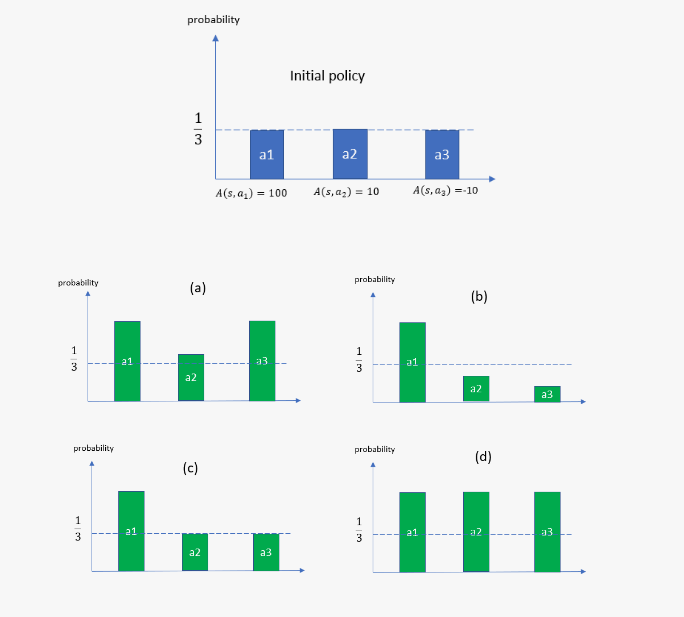
\includegraphics[scale=0.5]{./prob_13.png}
    \end{figure}

    \subsection{Answer}

    As given in the initial policy graph, the advantage function for $a_1$ is $100$, the advantage
    function for $a_2$ is $10$, and the advantage function for $a_3$ is $-10$. The initial probability
    of each action is $1/3$.\\

    After applying the policy gradient update, we expect the probability of each action to change
    as follows:

    \begin{itemize}
        \item The probability of $a_1$ will increase.
        \item The probability of $a_2$ will decrease.
        \item The probability of $a_3$ will decrease.
    \end{itemize}

    The only graph that satisfies these conditions is graph (b), therefore the answer is (b).

\end{homeworkProblem}

\end{document}